\documentclass[../thesis.tex]{subfiles}
\begin{document}
\chapter{Appendix}
\label{appendix}
Included here are the observable properties of the He100 and R175 models from
\citet{KasenWoosleyHeger2011}, including the observable flux and time visible 
(\RefFig{visibility2}) and the observable number for each feedback scenario 
(\RefFig{obsnumber2}).  These plots are to be compared to
\RefFig{visibility} and \RefFig{obsnumber} in \RefSec{JWSTobs}.  Both
cases may be detected with NIRCam beyond $z=15$ for deep exposures of
$10^6\,$s.

Also included is an extended version of \RefFig{area_obsR250} showing
the detectable number in observing campaigns totalling $10^6$, $10^7$
and $10^8\,$s for all four PISN models (\RefFig{area_obs}). Only
R250-type PISNe will be detectable above reshift 15, and R175- and
B200-type PISNe will only be detectable in observing campaigns
totalling greater than $10^7\,$s.

\begin{figure}
 \begin{center}
   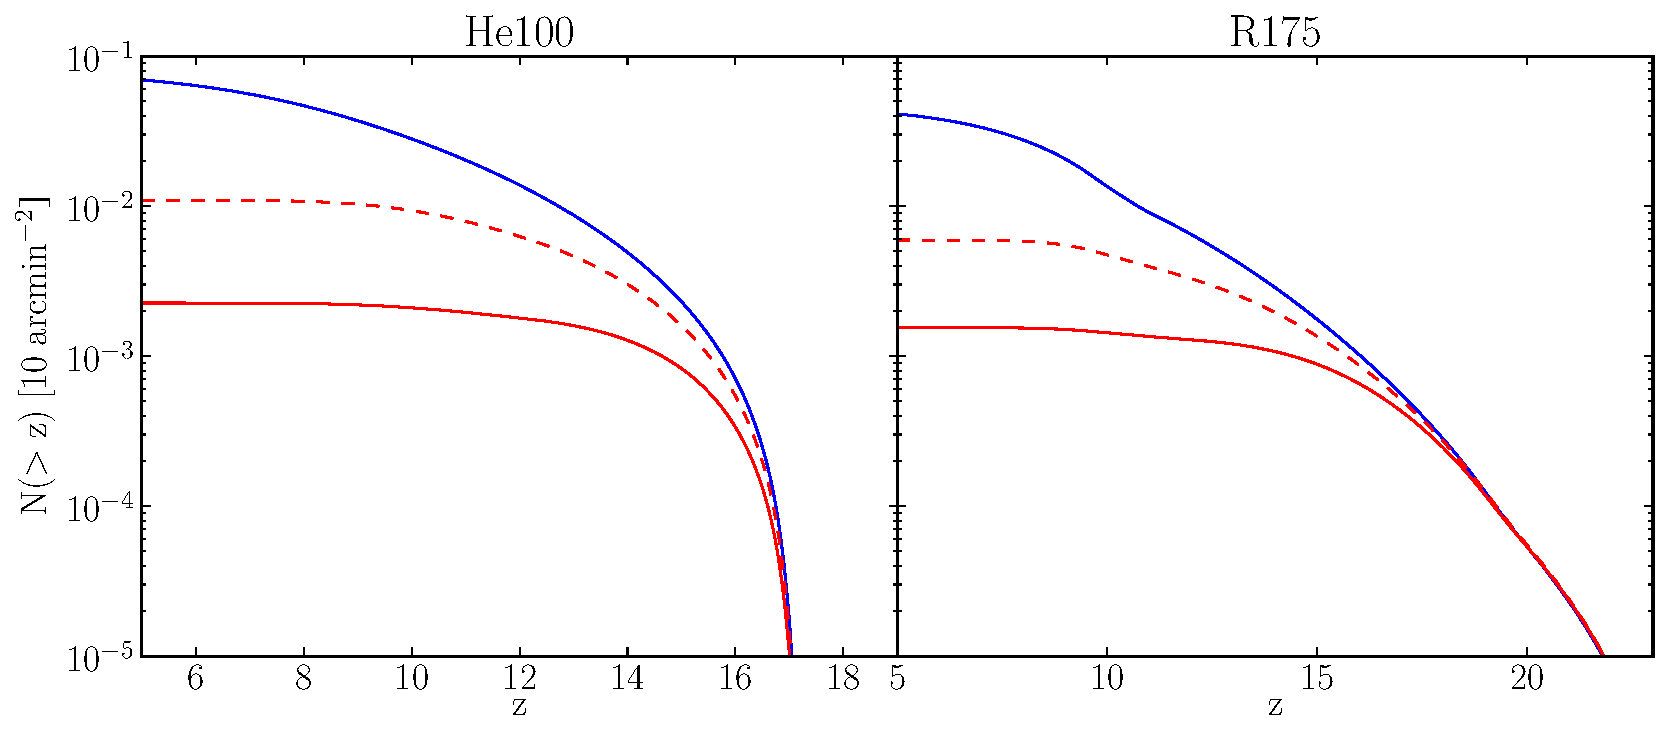
\includegraphics[width=\columnwidth]{observableNumber2}
   \caption{Upper and lower limits for the number of
     PISNe per JWST FoV above redshift $z$ with different feedback
     prescriptions. The observable numbers for a $10^6\,$s exposure
     assuming the He100 model are shown on the left; the R175 model is
     employed on the right. Solid blue lines show an upper limit
     to the observable number in the case of no feedback, solid red
     lines an estimate for the observable number in our conservative
     feedback scenario, and dashed red lines the number in the
     enhanced star formation case. Note that the x-axis is scaled
     independently in each panel.  }
   \label{obsnumber2}
 \end{center}
\end{figure} 

\begin{figure}
  \vspace*{\fill}
  \begin{center}
    \resizebox{15cm}{12cm}
              {\unitlength1cm
                \begin{picture}(15,12)
                  \put(0,6){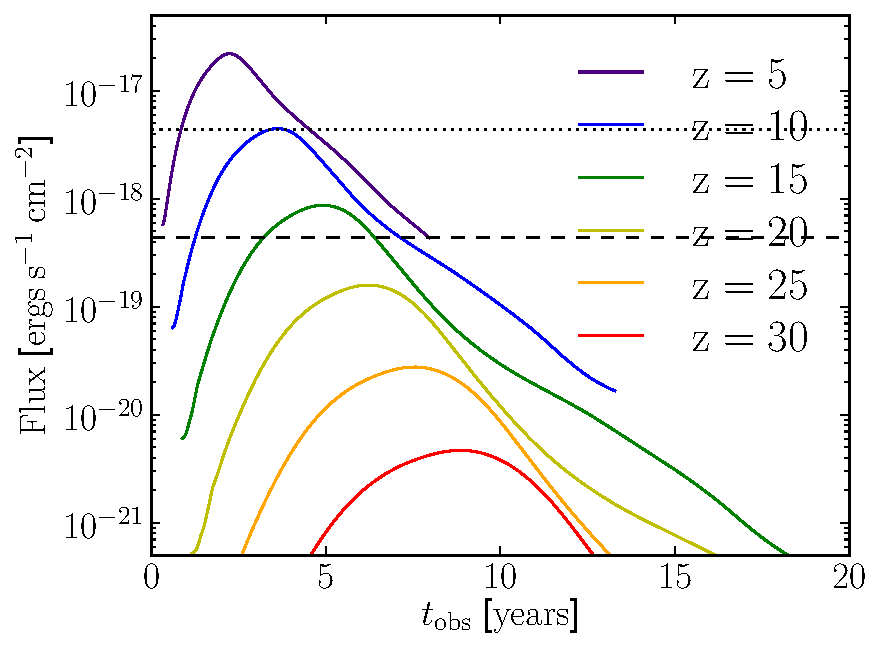
\includegraphics[width=7.5cm,height=6cm]{H100flux_F444W}}
                  \put(7.5,6){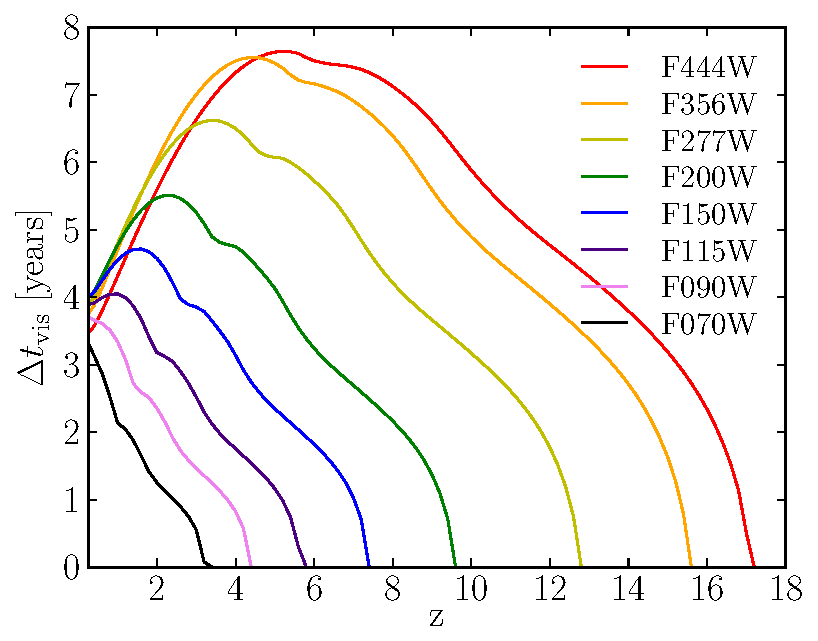
\includegraphics[width=7.5cm,height=6cm]{H100_t6}}
                  \put(0,0){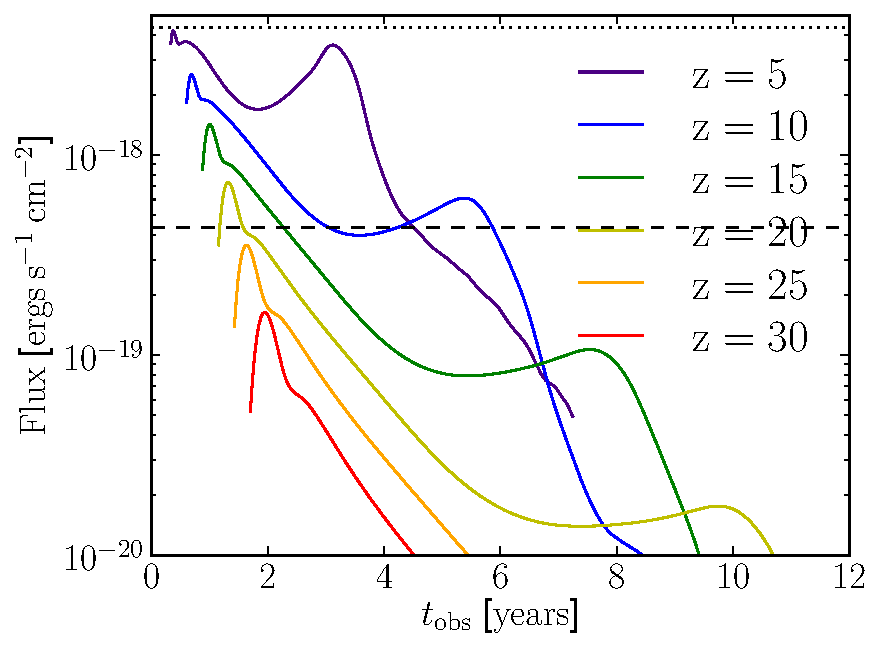
\includegraphics[width=7.5cm,height=6cm]{R175flux_F444W}}
                  \put(7.5,0){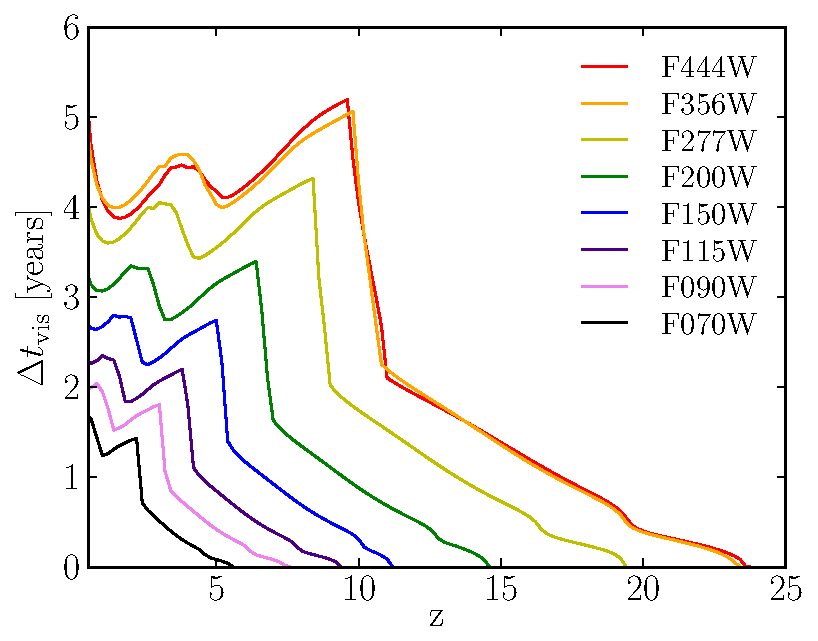
\includegraphics[width=7.5cm,height=6cm]{R175_t6}}
              \end{picture}}
              \caption{Left: Lightcurves for the
                \citet{KasenWoosleyHeger2011} He100 (top) and R175
                (bottom) models as they would be observed by JWST's
                F444W NIRCam filter at $z = 5, 10, 15, 20, 25 \:{\mathrm
                  and}\: 30$. The flux limits for a $10^6\,$s (dashed
                line) and $10^4\,$s (dotted line) exposure are shown
                for reference.  Right: The visibility time $\Delta
                t_{\mathrm vis}$ in years for He100 (top) and R175
                (bottom) as a function of redshift for each of the
                NIRcam wide filters. Note that the axes are scaled
                independently.}
              \label{visibility2}
  \end{center}
  \vspace*{\fill}
\end{figure}

\begin{figure}
  \vspace*{\fill}
  \begin{center}
    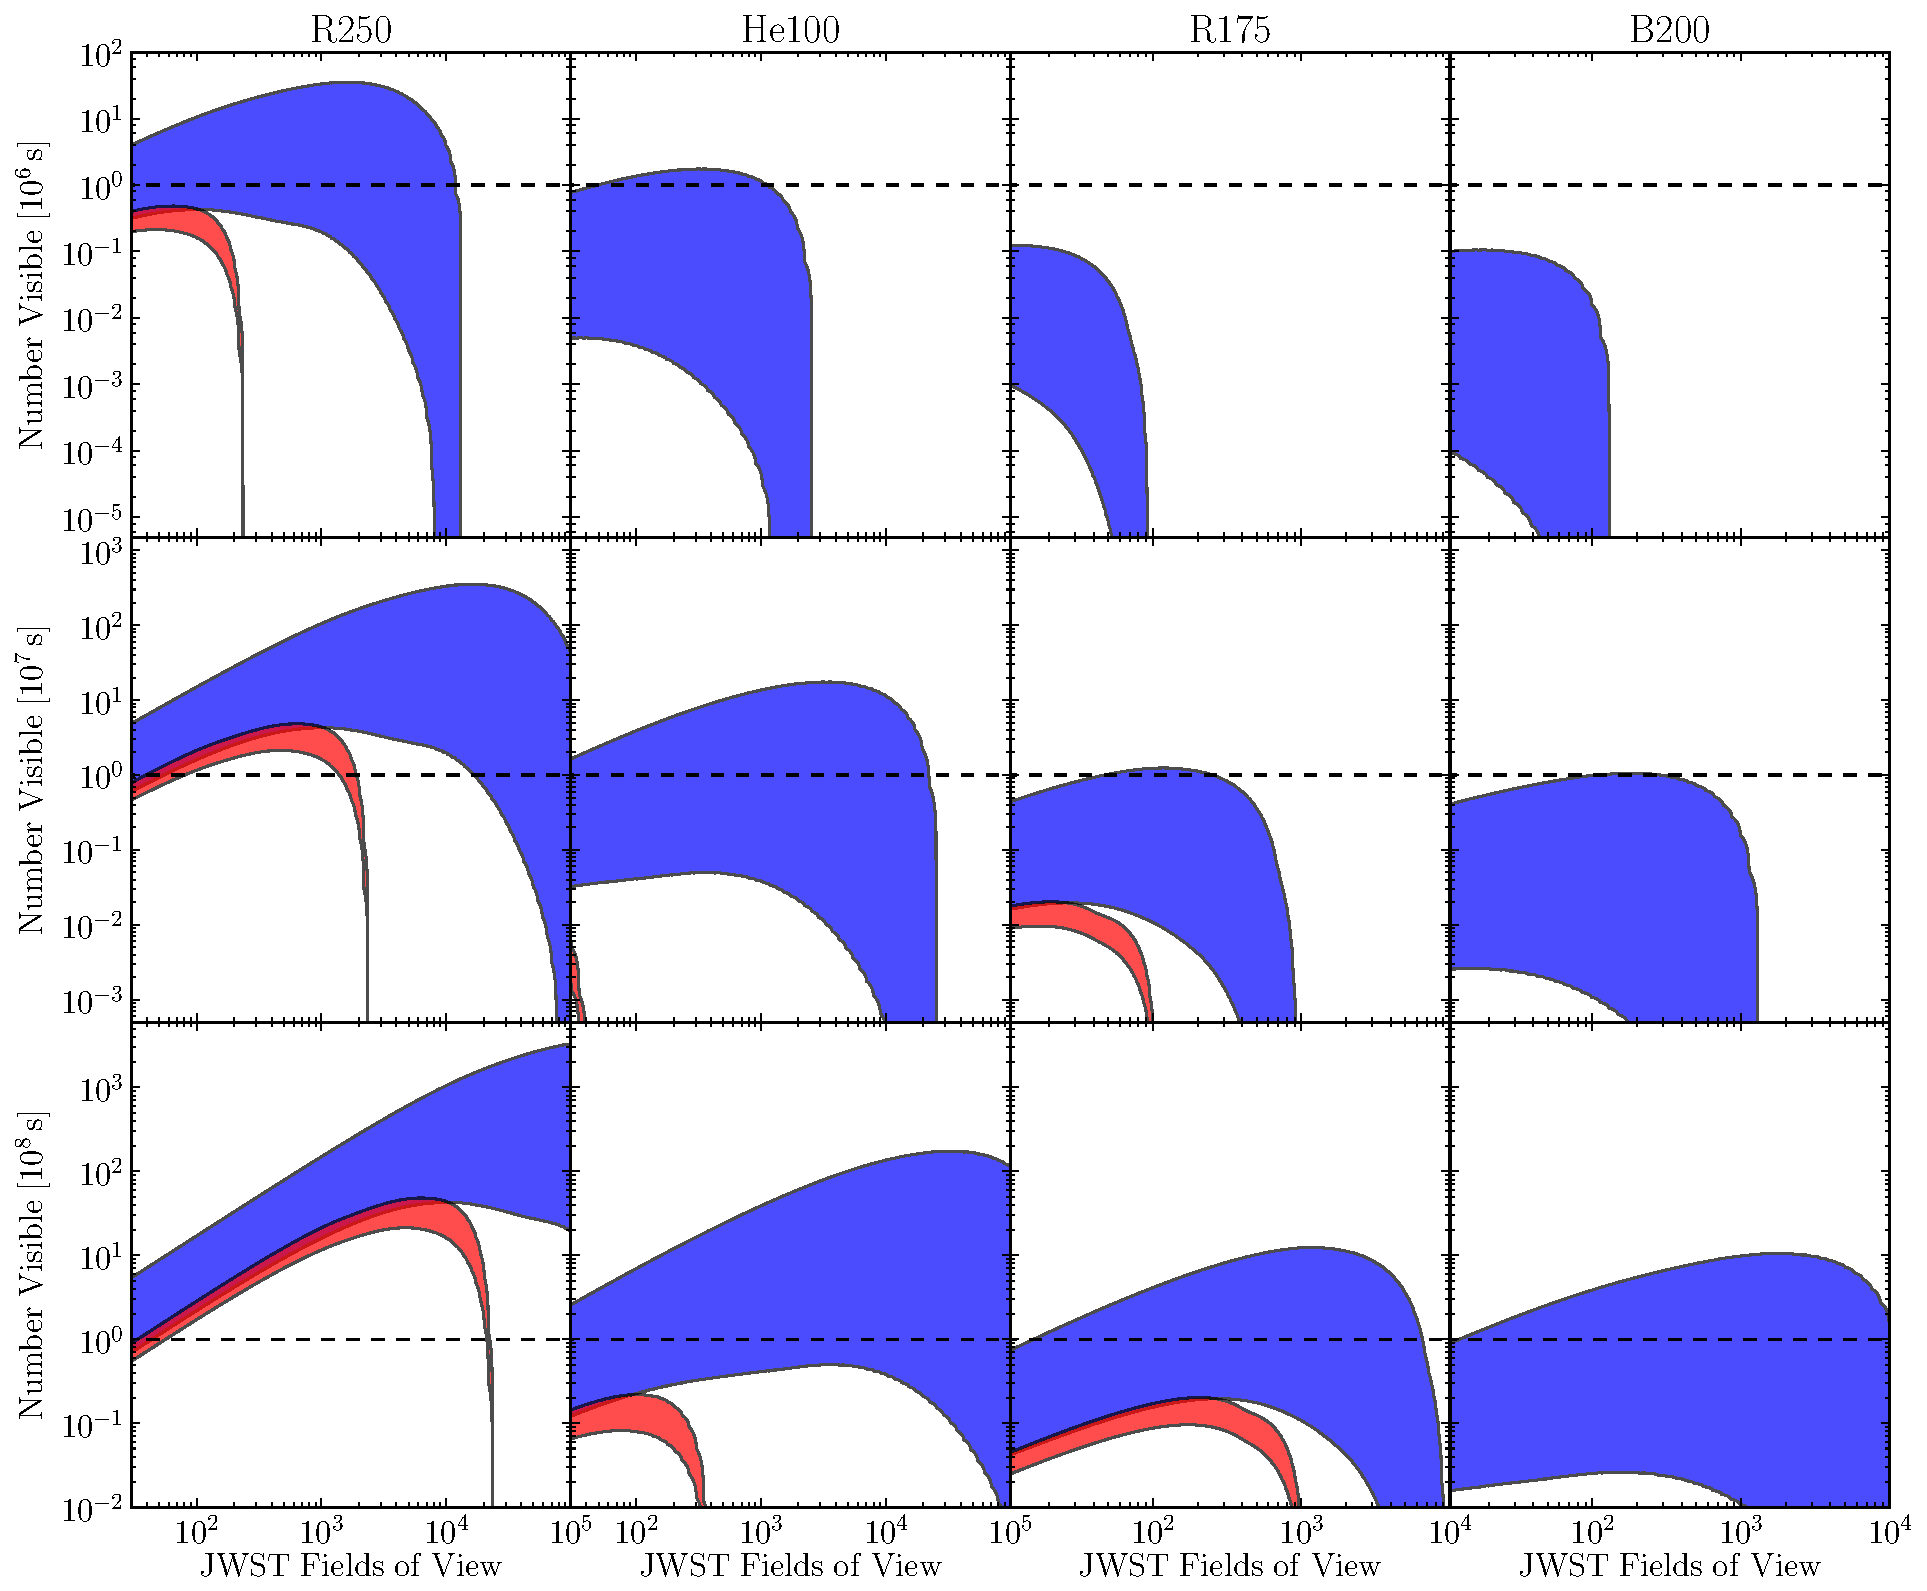
\includegraphics[width=\textwidth]{area_observability}
    \caption{The total number of PISNe observable with a
      campaign of $10^6$, $10^7$ and $10^8\,$s (from top to bottom) as
      a function of total survey area for a given PISN model.  In each
      case, the total campaign time is apportioned equally over the
      survey area to determine the exposure time for individual
      pointings.  The blue region represents all PISNe, the red only
      PISNe from $z>15$.  Upper boundaries correspond to the
      no-feedback upper limit to the PISN rate and lower boundaries to
      the conservative feedback case.  The dashed line marks one PISN
      visible. Note that not all axes are scaled the same.  }
    \label{area_obs}
  \end{center}
  \vspace*{\fill}
\end{figure} 
\end{document}